\documentclass[12pt,a4paper]{article}
\usepackage{lmodern}

%%%%%% TIKZ BIBLIOTHÈQUES %%%%%%
\usepackage{tikz}
\usetikzlibrary{3d}
\usepackage{pgfplots}
\usetikzlibrary{patterns}
\usepackage[european resistor, european voltage, european current]{circuitikz}
\usetikzlibrary{arrows,shapes,positioning}
\usetikzlibrary{decorations.markings,decorations.pathmorphing,
	decorations.pathreplacing}
\usetikzlibrary{calc,patterns,shapes.geometric}
\usepackage{tikz-3dplot}
\usetikzlibrary{matrix, calc, backgrounds, decorations.pathreplacing}
\usepackage{mathtools}
\usetikzlibrary{arrows.meta}

%%%%%%%%%%%%%%%%%%%%%%%%%%%%%%%

%%%%% GESTION DES RÉFÉRENCES %%%%%%
\usepackage{caption}
\pgfplotsset{compat=newest}
\usepackage{hyperref} % Crée des hyperliens pour le sommaire
\hypersetup{pdfborder=0 0 0} % Cache les cadres rouges autour des hyperliens
%%%%%%%%%%%%%%%%%%%%%%%%%%%%%%%%%%

%%% PAGE DE COUVERTURE %%%
\usepackage[utf8]{inputenc}
\usepackage[T1]{fontenc}
\usepackage[english]{babel}

%%% GESTION DES FIGURES %%%
\usepackage{float}      % Pour les figures à la place voulue UNIQUEMENT
\usepackage{graphicx}   % Pour inclure des figures
\usepackage{chngcntr}   % Bibli pour que la numérotation des figures dépende de la section
\usepackage{fancyhdr}
\usepackage{geometry}
\usepackage{titlesec}
\usepackage{tocloft} % package to adjust the appearance of the table of contents.
\usepackage{lipsum} % for sample text
\usepackage{glossaries}

\usepackage{amsfonts}   % Ensemble mathématique
\usepackage{amsmath}    % Environnement mathématique équation
\usepackage{tabularx}
\usepackage{colortbl}
\usepackage{array}
\usepackage{tcolorbox} % box coloré
\tcbuselibrary{skins} % Utilse pour faire Titres avancés: Personnaliser l'emplacement et l'apparence des titres des boîtes bien au-delà des capacités de base, comme dans l'exemple que je vous ai fourni, où le titre est placé en chevauchement sur le bord supérieur de la boîte.
\usepackage{mdframed}   % Box Théorèmes et définitions
\usepackage{xspace}     % Pour les redéfinitions de commandes
\usepackage{makecell}   % Pour des retours à la ligne dans une ligne de tableau
\usepackage{physics} % notation mathématique pour la physique 
\usepackage{subcaption}
\usepackage{amsthm}


%%% CONFIGURATION DE LA PAGE %%%
\usepackage{fancyhdr}
\usepackage{geometry}
\usepackage{titlesec}
\usepackage{systeme}
\usepackage{palatino} %%% style of the Latex
\usepackage{lastpage} 


\hypersetup{
    colorlinks=true,
    linkcolor=blue,     % Color for internal links (sections, equations, etc.)
    urlcolor=magenta,       % Color for URLs
    citecolor=red,    % Color for citations
    filecolor=green   % Color for file links
}
\hypersetup{pdfborder=0 0 0} % Cache les cadres rouges autour des hyperliens
%%%%%%%%%%%%%%%%%%%%%%%%%%%%%%%%%%


%%% Section
\newcommand{\hugetext}[1]{%
  \begin{flushleft}
    {\huge \textbf{#1}}
  \end{flushleft}
}




%%%
% Redefine the abstract environment
\makeatletter
\renewenvironment{abstract}{
    \if@twocolumn
      \section*{\abstractname}%
    \else
      \begin{center}%
        {\Huge\bfseries \leftline{\abstractname\vspace{-1em}}\vspace{0.3em}}%
      \end{center}%
	  \noindent

    \fi}
    {\if@twocolumn\else\endquotation\fi}
\makeatother
%%% Redefine the Contents


%%% color %%%

\definecolor{asparagus}{rgb}{0.53, 0.66, 0.42}
\definecolor{carminered}{rgb}{1.0, 0.0, 0.22}
\definecolor{darkpastelblue}{rgb}{0.47, 0.62, 0.8}
\definecolor{darkgray}{rgb}{0.66, 0.66, 0.66}
\definecolor{harvardcrimson}{rgb}{0.79, 0.0, 0.09}


%%%%CONFIG MATHS EQUATIONS
\usepackage{ mathrsfs } % FOR the H of the Hamiltionan

\newcommand{\id}[2]{ \hat{\mathbb{I}}_{#1}^{(#2)}}
\newcommand{\strope}[1]{ e^{i \pi \phi _{#1}}}
\newcommand{\stropeall}[1]{ e^{i \pi \displaystyle{ \sum_{l < #1}} f_l^\dagger f_l}}
\newcommand{\fd}[1]{ f^\dagger_{#1}}
\newcommand{\f}[1]{ f_{#1}}
\newcommand{\equalprop}[1]{ \underset{#1}{=}}     
\newcommand{\DFTterm}[4]{\sum_{#1=1}^{#2} #3 e^{-\frac{2i\pi #1#4}{#2}}}


%%% Size-adaptive math: {\textbackslash}leftX \ldots {\textbackslash}rightX
\newcommand{\bb}[1]{\left(#1\right)}                                        %% parantheses
\newcommand{\bc}[1]{\left[#1\right]}                                        %% brackets
\newcommand{\absv}[1]{\left|#1\right|}                                      %% absolute value
\newcommand{\absvsq}[1]{\absv{#1}^2}                                        %% absolute value squared
\newcommand{\meanv}[1]{\left\langle #1\right\rangle}                        %% mean value
\newcommand{\sumd}[2]{\displaystyle{\sum_{#1}^{#2}}}						%% sum 
%%% Fixed-size math (for quickly changing from adaptive style)
\newcommand{\Bb}[1]{\big(#1\big)}                                           %% big parantheses
\newcommand{\BB}[1]{\Big(#1\Big)}                                           %% Big parantheses
\newcommand{\Bc}[1]{\big[#1\big]}                                           %% big brackets
\newcommand{\BC}[1]{\Big[#1\Big]}                                           %% Big brackets
\newcommand{\Absv}[1]{\big|#1\big|}                                         %% big absolute value
\newcommand{\ABSV}[1]{\Big|#1\Big|}                                         %% Big absolute value
\newcommand{\Absvsq}[1]{\Absv{#1}^2}                                        %% big absolute value squared
\newcommand{\ABSVSQ}[1]{\ABSV{#1}^2}                                        %% Big absolute value squared
\newcommand{\Comm}[2]{\big[#1, #2\big]}                                     %% big commutator
\newcommand{\COMM}[2]{\Big[#1, #2\Big]}                                     %% Big commutator
\newcommand{\Meanv}[1]{\big\langle #1\big\rangle}                           %% big mean value
\newcommand{\MEANV}[1]{\Big\langle #1\Big\rangle}                           %% Big mean value


\newcommand{\braketop}[3]{\left\langle #1\middle|#2\middle|#3\right\rangle}  %% matrix element
\newcommand{\smallbraketop}[3]{\langle #1|#2|#3\rangle}                      %% small matrix element

%%% Special functions
\newcommand{\deltaf}[1]{\ensuremath{\delta\!\bb{#1}}\xspace}                    %% delta function
\newcommand{\thetaf}[1]{\ensuremath{\theta\!\bb{#1}}\xspace}                    %% theta function
\newcommand{\expf}[1]{\ensuremath{\operatorname{\text{exp}}\!\bb{#1}}\xspace}   %% exponential function
\newcommand{\ef}[1]{\ensuremath{\operatorname{e}^{#1}}\xspace}                  %% exponential function
\newcommand{\Refn}[1]{\ensuremath{\operatorname{Re}\!\bb{#1}}\xspace}           %% real part, function form
\newcommand{\Imfn}[1]{\ensuremath{\operatorname{Im}\!\bb{#1}}\xspace}           %% imaginary part, function form
\renewcommand{\Re}{\operatorname{Re}}                                           %% real part
\renewcommand{\Im}{\operatorname{Im}}                                           %% imaginary part

%%% Named states
\newcommand{\ketPsi}{\ket{\Psi}}
\newcommand{\ketpsi}{\ket{\psi}}
\newcommand{\ketphi}{\ket{\varphi}}
\newcommand{\ketup}{\ket{\uparrow}}      %% spin up
\newcommand{\ketdn}{\ket{\downarrow}}    %% spin down
\newcommand{\ketzero}{\ket{0}}
\newcommand{\ketone}{\ket{1}}
\newcommand{\ketg}{\ket{g}}              %% ground state
\newcommand{\kete}{\ket{e}}              %% excited state
\newcommand{\vac}{\ket{\text{vac}}}      %% vacuum
\newcommand{\up}{\uparrow}
\newcommand{\down}{\downarrow}

%%% Pauli matrices
\newcommand{\sx}[1]{\hat{\sigma}_x^{(#1)}}
\newcommand{\sy}[1]{\hat{\sigma}_y^{(#1)}}
\newcommand{\sz}[1]{\hat{\sigma}_z^{(#1)}}
\newcommand{\splus}[1]{\hat{\sigma}_+^{(#1)}}
\newcommand{\sminus}[1]{\hat{\sigma}_-^{(#1)}}

%%% Vectors
\newcommand{\vecr}{\vec{r}}
\newcommand{\vecrone}{\vec{r_1}}
\newcommand{\vecrtwo}{\vec{r_2}}
\newcommand{\vecrn}{\vec{r_N}}
\newcommand{\vecri}{\vec{r_i}}
\newcommand{\vecrj}{\vec{r_j}}
\newcommand{\vecR}{\vec{R}}
\newcommand{\vecx}{\vec{x}}
\newcommand{\vecy}{\vec{y}}
\newcommand{\vecz}{\vec{z}}
\newcommand{\vecxi}{\vec{x_i}}
\newcommand{\vecxj}{\vec{x_j}}
\newcommand{\veck}{\vec{k}}
\newcommand{\vecq}{\vec{q}}
\newcommand{\vecp}{\vec{p}}
\newcommand{\vecd}{\vec{d}}
\newcommand{\vecmu}{\boldsymbol{\mu}}
\newcommand{\vecsigma}{\boldsymbol{\sigma}}

%%% Differentiation
\newcommand{\partiald}[1]{\frac{\partial}{\partial #1}}               %% partial differentiation
\newcommand{\laplace}{\operatorname{\nabla^2}}                        %% laplace operator

%%% Integration
\newcommand{\integral}[1]{\int \! \mathrm{d} #1\,}                    %% integral
\newcommand{\integralb}[3]{\int\limits_{#1}^{#2} \! \mathrm{d} #3\,}  %% integral with boundaries
\newcommand{\integralf}[2]{\int \! \frac{\mathrm{d} #1}{#2}\,}        %% integral with fraction
\newcommand{\intvol}{\integral{^3r}}                                  %% integral over r space
\newcommand{\intvolp}{\integral{^3r'}}                                %% integral over r' space
\newcommand{\intvold}{\intvol\!\intvolp}                              %% double integral over space
\newcommand{\intk}{\integral{^3k}}                                    %% integral over k space
\newcommand{\intkp}{\integral{^3k'}}                                  %% integral over k' space
\newcommand{\intkn}{\integralf{^3k}{(2\pi)^3}}                        %% normalized integral over k space
\newcommand{\intkpn}{\integralf{^3k'}{(2\pi)^3}}                      %% normalized integral over k' space

%%% Special symbols
\newcommand{\hc}{\mathop{\text{h.c.}}}                               %% hermitian conjugate
\newcommand{\hamil}{\ensuremath{\operatorname{{\hat{H}}}}\xspace}    %% Hamilton operator
\newcommand{\hastobe}{\stackrel{!}{=}}                               %% has to be
\newcommand{\eqhat}{\mathrel{\widehat{=}}}                           %% corresponds to, is equivalent
\newcommand{\const}{\mathop{\text{const.}}}                          %% hermitian conjugate
\newcommand{\goesto}{\longrightarrow}                                %% maps to, asymptotically goes to
\newcommand{\basis}{\mathcal{B}}                                                %% maps to, asymptotically goes to

%%% Second quantization
\newcommand{\aop}{\ensuremath{a^{\vphantom\dagger}}\xspace}          %% annihilation operator a
\newcommand{\aopd}{\ensuremath{a^\dagger}\xspace}                    %% creation operator a

\newcommand{\bop}{\ensuremath{b^{\vphantom\dagger}}\xspace}          %% annihilation operator b
\newcommand{\bopd}{\ensuremath{b^\dagger}\xspace}                    %% creation operator b

\newcommand{\cop}{\ensuremath{c^{\vphantom\dagger}}\xspace}          %% annihilation operator c
\newcommand{\copd}{\ensuremath{c^\dagger}\xspace}                    %% creation operator c

\newcommand{\nop}{\ensuremath{n}\xspace}                             %% number operator

\newcommand{\psiop}{\ensuremath{\psi^{\vphantom\dagger}}\xspace}     %% field operator psi
\newcommand{\psiopd}{\ensuremath{\psi^\dagger}\xspace}               %% creation operator psi

\newcommand{\PsiOp}{\ensuremath{\Psi^{\vphantom\dagger}}\xspace}     %% field operator Psi
\newcommand{\PsiOpd}{\ensuremath{\Psi^\dagger}\xspace}               %% creation operator Psi

%%% Differences
\newcommand{\Dx}{\Delta x}
\newcommand{\Dy}{\Delta y}
\newcommand{\Dt}{\Delta t}


%%% Figures
\newcommand{\igopt}[2]{\includegraphics[#1]{#2}} %%! options, filename

\newcommand{\ig}[2]{\igopt{width=#1\columnwidth}{#2}} %%! width in units of textwidth, filename

\newcommand{\figopt}[4]{ %%! width, filename, caption, placement (h, t, ht)
	\begin{figure}[#4]
		\centering
		\ig{#1}{#2}
		\caption{#3}
		\label{fig:#2}
	\end{figure}
}

\newcommand{\fig}[3]{ %%! width, filename, caption
	\figopt{#1}{#2}{#3}{ht}
}

\newcommand{\doublefigopt}[8]{ %%! w1, f1, c1, w2, f2, c2, main caption, placement
	\begin{figure}[#8]
		\centering
		\subfloat[#3]{
			\ig{#1}{#2}
			\label{fig:#2}
		}
		\subfloat[#6]{
			\ig{#4}{#5}
			\label{fig:#5}
		}
		\caption{#7}
		\label{fig:#2_#5}
	\end{figure}
}

\newcommand{\doublefig}[7]{\doublefigopt{#1}{#2}{#3}{#4}{#5}{#6}{#7}{ht}} %%! w1, f1, c1, w2, f2, c2, main caption



\newcounter{prop}
\newcommand{\myprop}[3]{%
	\refstepcounter{prop}%
	\begin{tcolorbox}[
		enhanced,
		colback=white,
		colframe=darkpastelblue,
		fonttitle=\bfseries,
		title=Proposition \theprop: #1,
		attach boxed title to top left={yshift=-2mm, xshift=0.5cm},
		boxed title style={colback=darkpastelblue, size=small},
		sharp corners=all
		]
		\label{prop:#3} #2
	\end{tcolorbox}
}

\newcounter{thm}
\newcommand{\myth}[3]{%
	\refstepcounter{thm}%
	\begin{tcolorbox}[
		enhanced,
		colback=white,
		colframe=harvardcrimson,
		fonttitle=\bfseries,
		title=Theorem \thethm: #1,
		attach boxed title to top left={yshift=-2mm, xshift=0.5cm},
		boxed title style={colback=harvardcrimson, size=small},
		sharp corners=all
		]
		\label{thm:#3}#2
	\end{tcolorbox}
}

\newcounter{coro}
\newcommand{\mycoro}[3]{%
	\refstepcounter{coro}%
	\begin{tcolorbox}[
		enhanced,
		colback=white,
		colframe=aurometalsaurus,
		fonttitle=\bfseries,
		title=Corollary \thecoro: #1,
		attach boxed title to top left={yshift=-2mm, xshift=0.5cm},
		boxed title style={colback=aurometalsaurus, size=small},
		sharp corners=all
		]
		\label{coro:#3}#2
	\end{tcolorbox}
}

\newcounter{defn}
\newcommand{\mydef}[3]{%
	\refstepcounter{defn}%
	\begin{tcolorbox}[
		enhanced,
		colback=white,
		colframe=asparagus,
		fonttitle=\bfseries,
		title=Definition \thedefn: #1,
		attach boxed title to top left={yshift=-2mm, xshift=0.5cm},
		boxed title style={colback=asparagus, size=small},
		sharp corners=all
		]
		\label{def:#3} #2
	\end{tcolorbox}
}

\newcounter{lem}
\newcommand{\mylemma}[3]{% tilte, text, label
	\refstepcounter{lem}%
	\begin{tcolorbox}[
		enhanced,
		colback=white,
		colframe=orange,
		fonttitle=\bfseries,
		title=Lemma \thelem: #1,
		attach boxed title to top left={yshift=-2mm, xshift=0.5cm},
		boxed title style={colback=orange, size=small},
		sharp corners=all
		]
		\label{lem:#3} #2
	\end{tcolorbox}
}

\newcounter{postulat}
\newcommand{\mypostulat}[3]{%
	\refstepcounter{postulat}%
	\begin{tcolorbox}[
		enhanced,
		colback=white,
		colframe=darkgray,
		fonttitle=\bfseries,
		title=Postulate \thepostulat: #1,
		attach boxed title to top left={yshift=-2mm, xshift=0.5cm},
		boxed title style={colback=darkgray, size=small},
		sharp corners=all
		]
		\label{postulat:#3} #2
	\end{tcolorbox}
}

% Reference commands
\newcommand{\refth}[1]{\hyperref[#1]{Theorem~\ref*{#1}}}
\newcommand{\refprop}[1]{\hyperref[#1]{Proposition~\ref*{#1}}}
\newcommand{\refcoro}[1]{\hyperref[#1]{Corollary~\ref*{#1}}}
\newcommand{\refdef}[1]{\hyperref[#1]{Definition~\ref*{#1}}}
\newcommand{\reflem}[1]{\hyperref[#1]{Lemma~\ref*{#1}}}
\newcommand{\refpostulat}[1]{\hyperref[Postulat:#1]{postulate~\ref*{#1}}}
\newcommand{\myeqref}[1]{\hyperref[#1]{Equation~\ref*{#1}}}





%%% CONFIGURATION DE LA PAGE %%%
\geometry{
	top=2cm,
	bottom=2cm,
	left=2cm,
	right=2cm,
	headheight=15pt,
	includeheadfoot
}


% Define the total number of pages in Roman and Arabic
\newcounter{romanpages}
\setcounter{romanpages}{6} % Set this to the actual number of Roman numeral pages

\newcounter{arabicpages}
\setcounter{arabicpages}{20} % Set this to the actual number of Arabic numeral pages

% Define Roman page style
\fancypagestyle{romanstyle}{
	\fancyhf{}
	\renewcommand{\headrulewidth}{0.5pt}
	\fancyhead[L]{\textbf{Quantum information}}
	\fancyfoot[L]{\textbf{page \thepage} / \textcolor{blue}{\textbf{\Roman{romanpages}}}} % Page number on the left
	\fancyfoot[R]{{Internship USACH - Quantum information}} % Custom text on the right
}

% Define Arabic page style
\fancypagestyle{arabicstyle}{
	\fancyhf{}

	\renewcommand{\headrulewidth}{0.5pt}
	\fancyhead[L]{\textbf{Quantum information}}
	\fancyfoot[L]{\textbf{page \thepage} / \textcolor{blue}{\textbf{\arabic{arabicpages}}}} % Page number on the left
	\fancyfoot[R]{{Internship USACH - Quantum information}} % Custom text on the right
}

% Plain page style
\fancypagestyle{plain}{
	\fancyhf{}
	\renewcommand{\headrulewidth}{0.5pt}
	\fancyhead[L]{\textbf{Quantum information}}
	\fancyfoot[L]{\textbf{page \thepage} / \textcolor{blue}{\textbf{\Roman{romanpages}}}} % Page number on the left
	\fancyfoot[R]{{Internship USACH - Quantum information}} % Custom text on the right
}

\renewcommand{\footrule}{\hrulefill} % Draw horizontal line

% Configuration des titres de sections
\titleformat{\section}[hang]{\normalfont\huge\bfseries}{\thesection.}{0.5em}{}

\setlength{\parskip}{0.4em}
\title{Entanglement in a spin chain}
\author{\textbf{Vincent MARAIS}}

\newpage

\begin{document}
%%% FIRST PAGE
	\input{first_page/title.tex}
%%%% REPORT FORMAL

\newpage

\pagestyle{romanstyle}
\pagenumbering{Roman}
%%%%% ABSTRACT
\begin{abstract}
	\lipsum[1] % replace with your abstract

    Quantum information XY-$\Gamma$ chain 

\end{abstract}

\underline{\textbf{Keywords :}}

\newpage
%%%% Acknowledgements
\section*{Acknowledgements}
\newpage



\newpage
%%%% List of tableofcontents

		
\tableofcontents


\newpage

		\listoffigures

\newpage
		
		\listoftables
		\addcontentsline{toc}{section}{List of Figures} 





\newpage
\pagestyle{arabicstyle}
\pagenumbering{arabic}
\section{Introduction}

Quantum entanglement, a fundamental feature of quantum mechanics, 
was first recognized in the early 20th century by Einstein, 
Podolsky, Rosen, and Schrödinger \cite{horodecki_quantum_2009}. This phenomenon describes 
a situation where the quantum states of two or more particles 
become intertwined, such that the state of one particle cannot 
be described independently of the state of the other, 
no matter the distance separating them. 



Entanglement become a practical resource 
in quantum information science, 
underpinning technologies such as quantum cryptography \cite{pirandola_advances_2020}, 
quantum teleportation \cite{bennett_teleporting_1993}, and quantum computing \cite{whitfield_quantum_2022}. 
These applications exploit entanglement 
to perform tasks that are impossible 
with classical systems.

Despite its utility, entanglement is a fragile and complex phenomenon, 
challenging to detect and manipulate. 
The study of entanglement involves understanding 
its properties, methods for its detection, and 
strategies for its quantification and manipulation. 
These efforts are crucial for advancing our ability 
to harness entanglement for practical applications, 
ensuring that it can be effectively used as a resource
in quantum communication and computation.



The work presented a quantum simulation of a specific
model of 1D lattice of \textbf{qubits} (quantum bit) a quantum system 
capable of existing in two states, such as 
the spin-up \(\ket{\uparrow}\) and spin-down 
\(\ket{\downarrow}\) states of an electron call Heisenberg XY model \cite{van_der_sijs_heisenberg_1993}
and with a Dzyaloshinskii-Moriya interaction (DMI) \cite{moriya_anisotropic_1960,dzyaloshinsky_thermodynamic_1958}. Finally 
a protocol to accelerating the entanglement in this lattice. 




\newpage
	

\section{Methodology}
The goal here is to computed the time evolution of the concurrence $C(\rho (t))$ in the lattice 
\refig{fig:Schematic of the lattice of the spin chain}
with the Hamiltonian of the XY and DMI.
For that with have two approch a numerical approch with the language of programmation Python and the 
analytical approch.

\subsection{Numerical approch}

To simulation the evolution of the concurrence \refdef{def: concurrence} we have to computed the 
density matrix but the necessery 
condition to computed the density matrix $\rho(t)$ in to found 
the state at the time $t$ the quantum system. For that 
we use the postulat of the evolution of the quantum system the Schrodïnger equation \cite{cohen-tannoudji_quantum_2019}. 

\begin{equation}\label{eq: Schrodïnger eq}
    \forall t \in \mathbb{R}_+, \ i \hbar \partial_t \ket{\psi(t)} = \hamil(t) \ket{\psi (t)} 
\end{equation}

Now let explain a generic algorithm to solve the Schrodïnger equation.

First let introduce the evolution operator $ \opevolution{t_0}$ which maps $ \ket{\psi(t_0)}$ the inital state of 
the system into $\ket{\psi(t)} $  

\begin{equation}\label{def : evolution operator}
   \forall t \in \mathbb{R}_+, \ \ketpsit = \opevolution{t_0}  \ket{\psi(t_0)} 
   \text{ with  } \ \opevolution{t_0} \opevolution{t_0}^\dagger = \opevolution{t_0}^\dagger \opevolution{t_0} = \text{id}  
\end{equation}

where $\text{id}$ is the identity function and $\opevolution{t_0}^\dagger$ is the adjoint of $\opevolution{t_0}$.
Now we start by considering a Hamiltonian \( \hamil(t) \) which is piecewise constant, i.e.,


\begin{equation}\label{prop: hypothese Hamiltionan}
    \forall j \in \mathbb{N}, \  \hamil(t) = \hamil(t_j) \quad \text{for} \quad t_j < t < t_{j+1},     
\end{equation}

where \( t_j \) are time steps at which the Hamiltonian changes suddenly.
\graphli{0.7}{methodology/constante_H.pdf}{Schematic of the \refprop{prop: hypothese Hamiltionan}}{hypothese Hamiltionan}

But now with the \refprop{prop: hypothese Hamiltionan}, the \refdef{def : evolution operator} and the \myeqref{eq: Schrodïnger eq}
we can express the $\opevolution{t_0}$ like this :

\begin{equation}
    \opevolution{t_0} = e^{-i \hamil (t-t_0)/\hbar}
\end{equation}



If we know the state of the quantum system at \( t_0 \), then we can compute the state quantum system at time \( t_n \) with $n > 0$ as:

\begin{align*}
    \ketpsitime{t_1} &= e^{-i \hamil (t_0) (t_1-t_0)/\hbar} \ketpsitime{t_0} \\
    \ketpsitime{t_2} &= e^{-i \hamil (t_1) (t_2-t_1)/\hbar} \ketpsitime{t_1} =  e^{-i \hamil(t_1) (t_2-t_1)/\hbar} 
    e^{-i \hamil(t_0) (t_1-t_0)/\hbar} \ketpsitime{t_0}\\
    &\vdots \\
    \ketpsitime{t_n} &= e^{-i \hamil(t_{n-1}) (t_n-t_{n-1})/\hbar} \ketpsitime{t_{n-1}} \cdots  e^{-i \hamil(t_{0}) (t_2-t_1)/\hbar} 
    e^{-i \hamil (t_1-t_0)/\hbar} \ketpsitime{t_0}
\end{align*}

Let us consider equally spaced time intervals:

\[
t_j = t_0 + j \Delta t.
\]

So the state of the quantum system at the time $t_n$ is  :
\begin{equation} \label{eq: expression state t_n}
   \forall n \in \mathbb{N}^*, \  \ketpsitime{t_n} = \prod_{i=0}^{n-1} e^{-i \hamil(t_{i}) \Delta t /\hbar} \ketpsitime{t_0}
\end{equation}

Notice the temporal order of operators \( \mathcal{U}(t_j, t_{j-1}) \) with \( t_j > t_{j-1} \). Operators later in time appear to the left.

So with deduce this algorithm to solve the Schrodïnger equation :
\begin{algorithm}[H]
    \caption{Solve Time-Dependent Schrödinger Equation}
    \begin{algorithmic}[1]
    \Procedure{solve}{$n: \text{integer}, t_f: \text{integer}, \text{Hamil: function}, \ketpsitime{t_0}: \text{array}$}
    \State $\Delta t \gets \frac{t_f}{n}$
    \State $\text{times} \gets \text{linspace}(0, t_f, n)$
    \State $\text{state\_t} \gets \text{empty list}$
    
    \For{$j = 0$ \textbf{to} $\text{length of times} - 1$}
        \State $\hamil(t_j) \gets \text{Hamil(times}[j])$
        \State $\mathcal{U}(t_{j+1}-t_j) \gets \text{matrix\_exponential}\left(-i \times \hamil(t_j) \times \Delta t \right)$
        \State $\ket{\psi(t_{j+1})} \gets \text{matrix\_dot\_product}(\mathcal{U}(t_{j+1}-t_j), \ket{\psi(t_0)})$
        \State \text{append } $\ket{\psi(t_{j+1})}$ \text{ to state\_t}
        \State $\ket{\psi(t_0)} \gets \ket{\psi(t_{j+1})}$
    \EndFor
    
    \State \Return $\text{state\_t}$
    \EndProcedure
    \end{algorithmic}
\end{algorithm}

\newpage 


Now we can compute the density matrix at the time $t$ but here if the length of the lattice is $L>1$ we can not 
compute the $C(\rho (t))$ according at the \refdef{def: concurrence} the concurrence in between only two qubits but if $L>1$ 
we have more of 2 qubits in the lattice so we can't use the  of the concurrence. 
Let see a example with 3 qubits to solve the problem in the figure :

\begin{figure}[h!]
    \centering
    \begin{subfigure}[b]{0.3\textwidth}
        \centering
        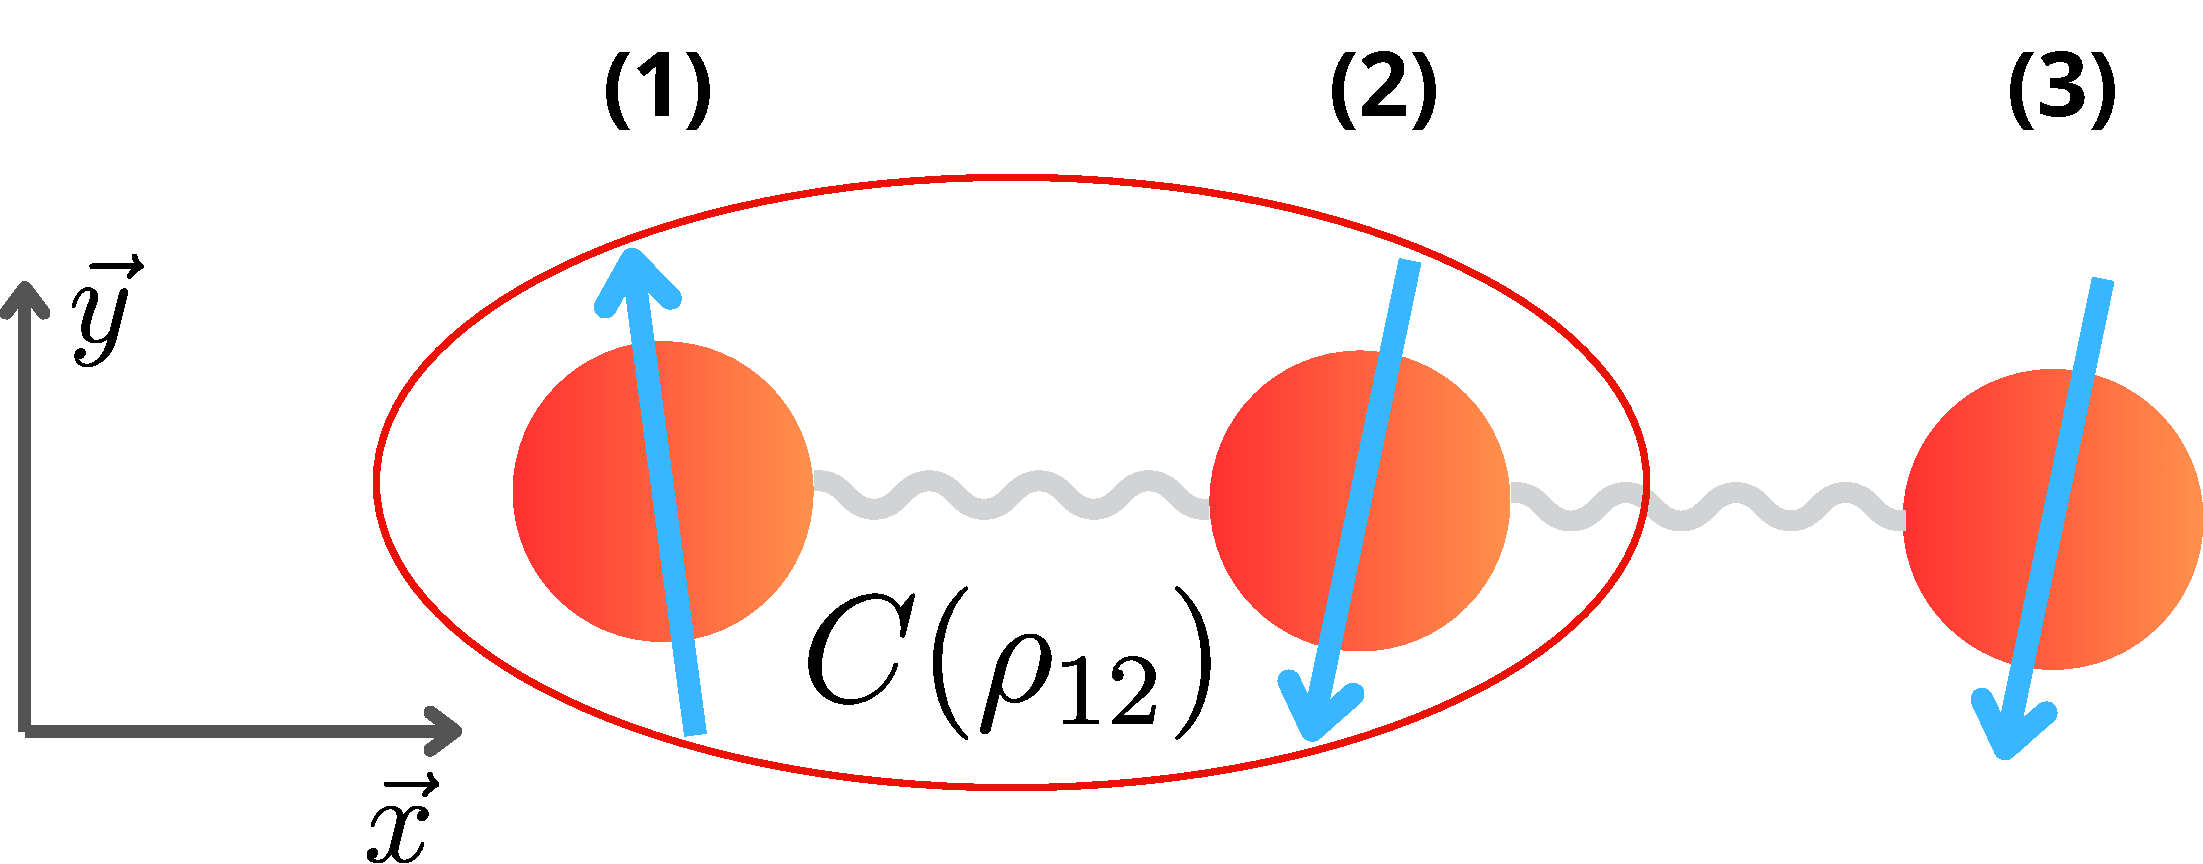
\includegraphics[width=\textwidth]{methodology/partial_trace_1.pdf}
        \caption{\centering Concurrence between the qubit (1) and (2)}
        \label{fig:Concurrence between the qubit (1) and (2)}
    \end{subfigure}
    \hfill
    \begin{subfigure}[b]{0.3\textwidth}
        \centering
        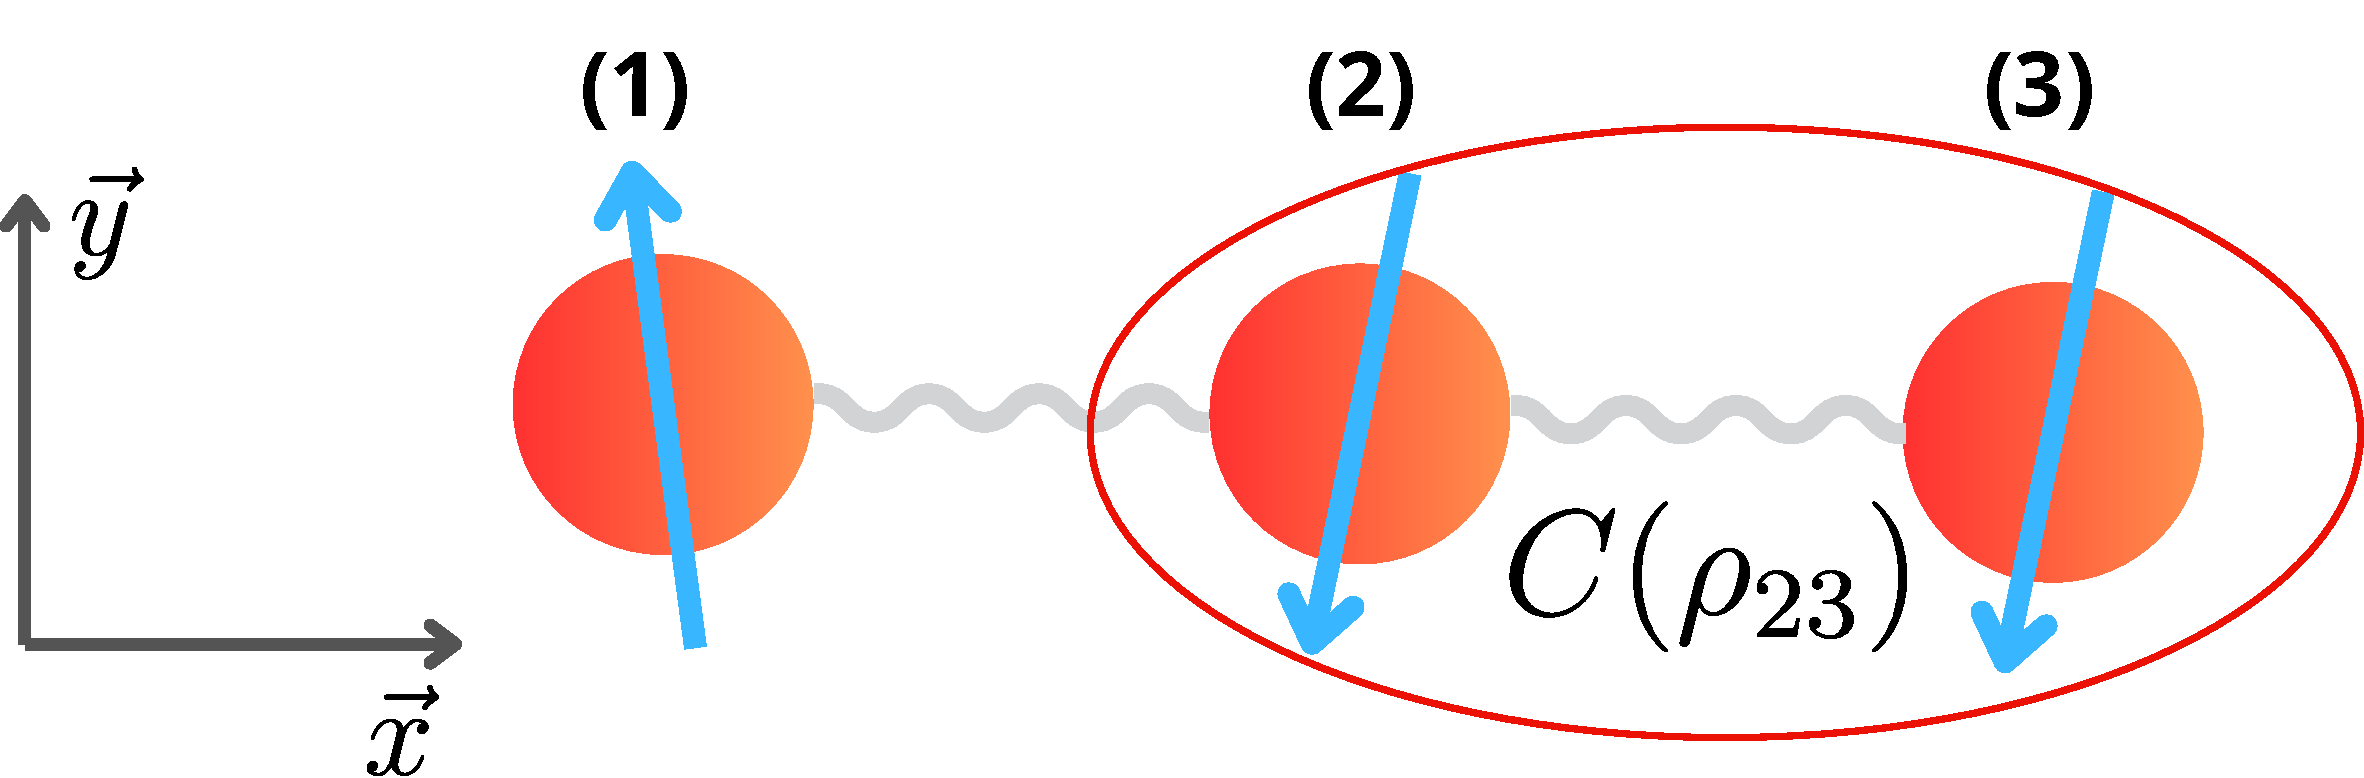
\includegraphics[width=\textwidth]{methodology/partial_trace_2.pdf}
        \caption{\centering Concurrence between the qubit (2) and (3)}
        \label{fig:Concurrence between the qubit (2) and (3)}
    \end{subfigure}
    \hfill
    \begin{subfigure}[b]{0.3\textwidth}
        \centering
        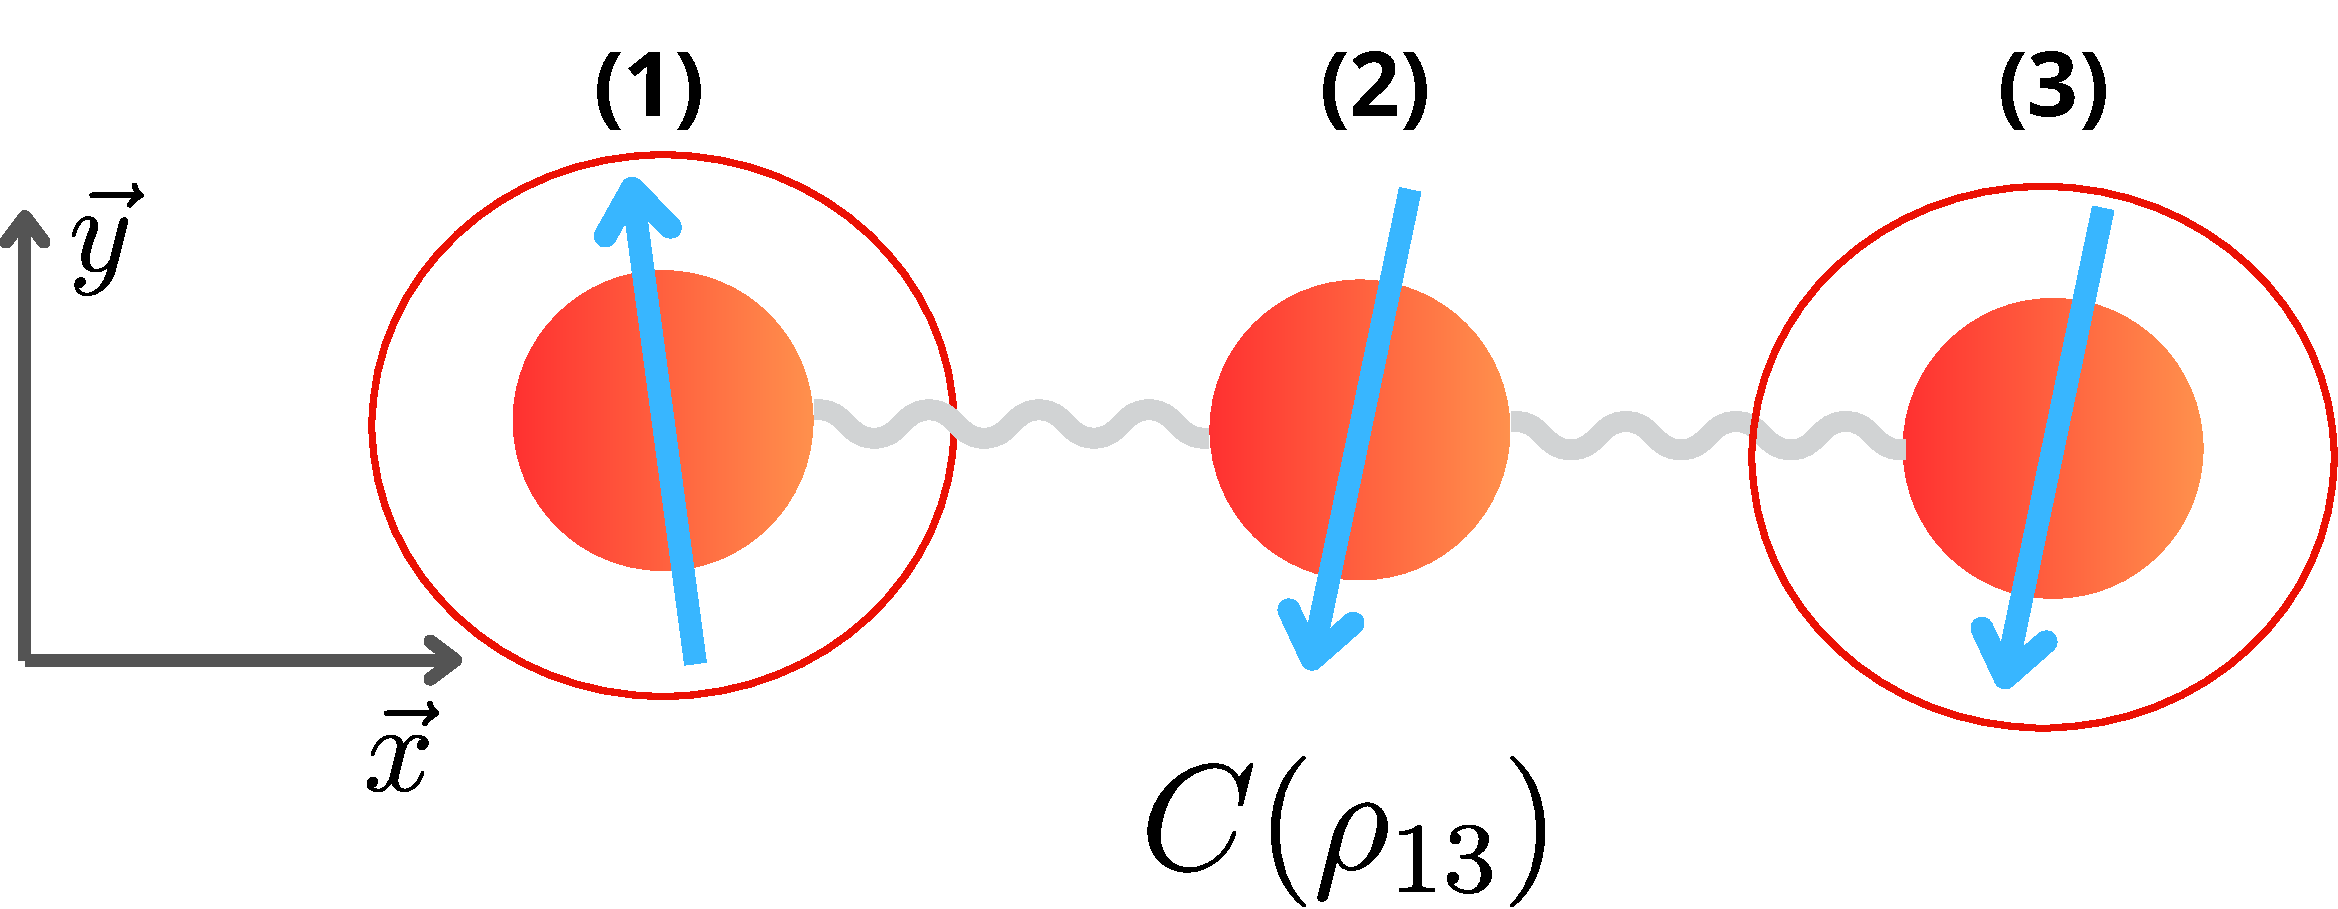
\includegraphics[width=\textwidth]{methodology/partial_trace_3.pdf}
        \caption{\centering Concurrence between the qubit (1) and (3)}
        \label{fig:Concurrence between the qubit (1) and (3)}
    \end{subfigure}
    \caption{Problem of calculation of the concurrence for many qubits}
    \label{fig:partial_traces}
\end{figure}



We understand we the \refig{fig:partial_traces} with have to a isolate the pair of the qubit and computed the density matrix of the 
couple of qubit note $\rho_{ij}$ where $i \neq j \text{ and } (i,j) \in \mathbb{N}^*$, for that we will use a mathematical tool call the partial
trace \cite{bradley_at_2020} 

\mydef{Partial trace}{
Let take a system of $L+1$ quantum system so 

\begin{equation}
    (i,j) \in (\mathbb{N}^*)^2 \text{ and } i \neq j , \ \rho_{ij} = \sumd{i=1}{\dim(A)} \bra*{e_i} \rho \ket{e_i}
\end{equation}

}{}

Let do a example
For example if we want to compute the density matrix of the system of the qubit (1) and (2) schematic 
in the \refig{fig:Concurrence between the qubit (1) and (2)} 








\newpage 

\section{Results And Discussion}
Results And Discussion

\newpage

\bibliographystyle{plain}
\bibliography{Intership_USACH.bib}
\end{document}